\chapter{Methods and data}

The following subsections provide a sufficient overview on the numerical model and analysis tools used for the presented work to allow a conclusive interpretation of the results thereafter.

\section{CORAL temperature measurements} 
\label{sec:coral}

\textcite{kaifler_compact_2021} provide a more extensive summary on CORAL's setup and observation,


\section{(ERA5 reanalysis data)}

% eventually comment on observational filter of satellite measurments from with figure from Hindley



\section{Spectral filtering}
% FFT

refer to filtering described in Kruse paper and from Vera
but mention equations

Gaussian filter vs. butterworth filter

and describe butterworth filter for CORAL data

\section{Wavelet Analysis}

The wavelet analysis described by \textcite{torrence_practical_1998} is used for deriving horizontal and vertical wavelengths of GWs in the idealized numerical simulations. 





\begin{equation}
    \mathcal{F}_x =  \rho_0 \int_{-\infty}^{\infty} (u'\omega' + f v' \eta') dx + f \int_{-\infty}^{\infty} \rho' v' \eta' dx
    \label{equ:morlet}
\end{equation}

The normalization with the variance of the data $\sigma^2$ gives a measure of the power relative to white noise. 

Then there is red noise too.


\begin{figure*}[tbp]
    \centering
    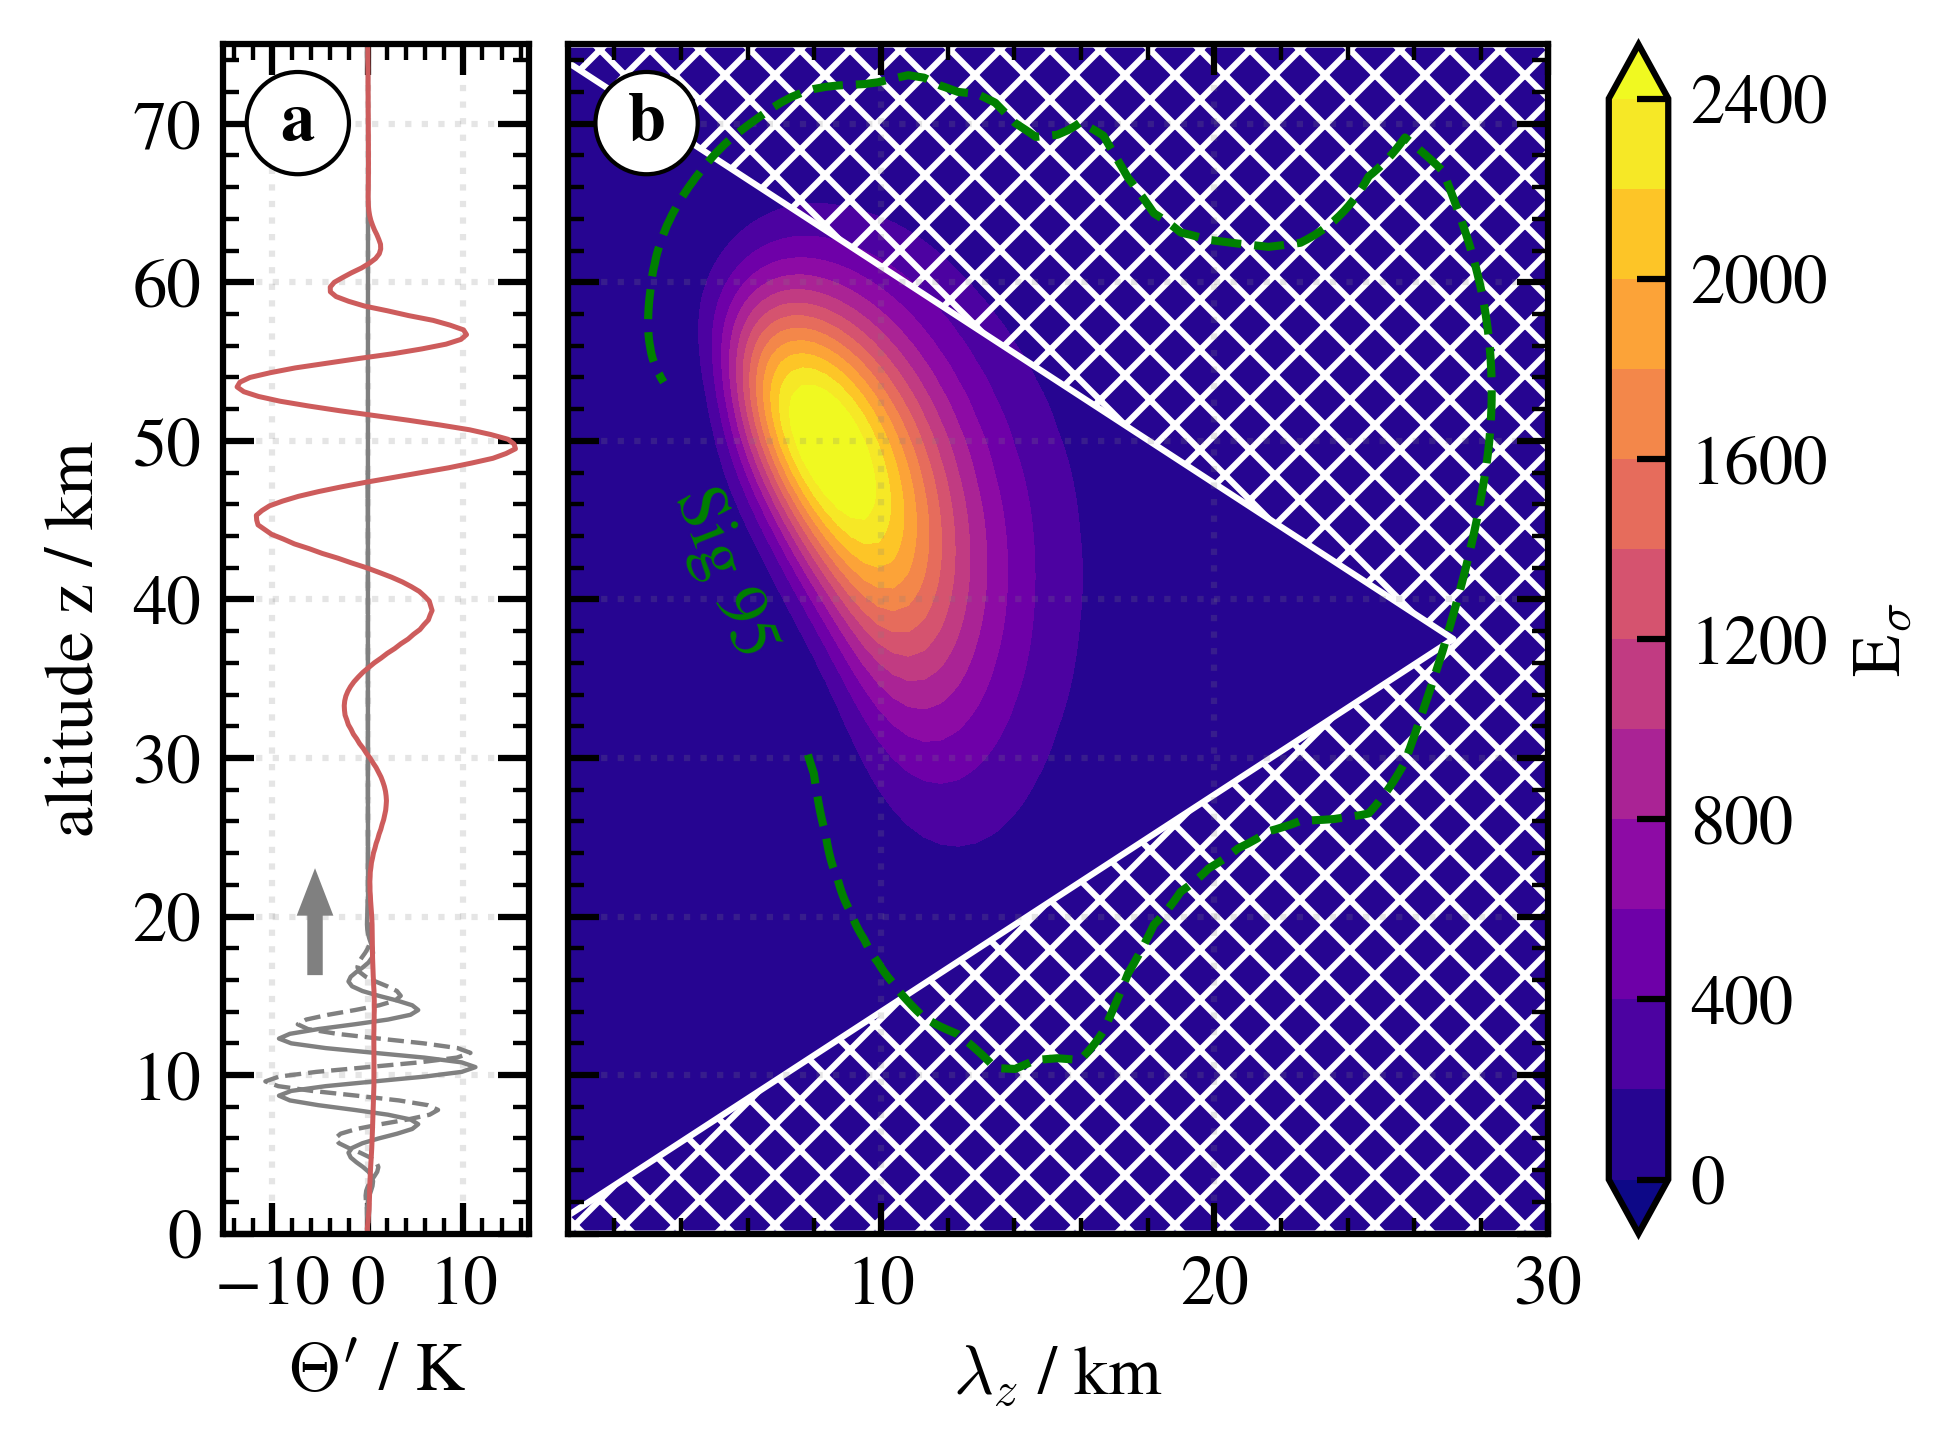
\includegraphics[width=0.99\textwidth]{figures_methods/waveletAna_power_spectrum.png}
    \caption{}
    \label{fig:wavelet_example}
\end{figure*}


% Mithilfe der Wavelet-Transformation können aus einer Datenreihe nicht nur die auftre- tenden Frequenzen extrahiert werden, sondern auch Informationen darüber, in welchen Abschnitten der Datenreihe welche Frequenzen dominant sind. Als Basisfunktionen wer- den dabei räumlich lokalisierte Wellen, sogenannte Wavelets, verwendet.

% Folgenden wird die Wavelet-Analyse anhand einer Datenreihe f(z) erläutert, die ent- lang einer räumlichen Achse z variiert. Dabei wird auf die Beschreibung in Torrence & Compo (1998) zurück gegriffen. Die Autoren stellen auf der Website http://atoc.colorado.edu/research/wavelets/ Software zur Anwendung der Wavelet-Ana- lyse zur Verfügung, die in dieser Arbeit verwendet wurde.
% Hier wurde das Morlet-Wavelet ψ0(η) benutzt, das von einem dimensionslosen Ortspa- rameter η abhängt und als
% ψ0(η) = π−1/4 ei ω0η e−η2/2 (3.39)
% definiert ist. Real- und Imaginärteil von ψ0 sind in Abbildung 3.6a dargestellt. Wird f(z) als eine Datenreihe fj diskretisiert, die bei konstanter Intervallgröße ∆z auf einem Gitter mit Index j = 0,...,N−1 definiert ist, kann daraus die kontinuierliche Wavelet- Transformation Wn(s) ermittelt werden. Diese ist definiert als Faltung von fj mit einer skalierten und verschobenen Version der Wavelet-Funktion:
% N−1 Wj(s) = �� fj′ ψ∗
% ��(j′ −j)∆z�� s
% (3.40) die komplex konjugierte normierte Wavelet-Funktion ψ0.
%  Hierbei ist ψ
% ∗
% ���� ∆z ��1/2 ��∗ = s ψ0
% j′=0
%  Indem die Wavelet-Skala s variiert und ψ∗ entlang des Ortsindex j verschoben wird, kann ein Bild rekonstruiert werden, das sowohl die Amplitude einzelner Merkmale des Signals zeigt als auch die Variation der Amplitude mit dem Ort.
% Für jede Skala s muss Gleichung (3.40) N-mal angewandt werden, damit die kontinu- ierliche Wavelet-Transformation approximiert wird. Diese Berechnung erfolgt deutlich schneller im Fourier-Raum, wo die Wavelet-Transformation gleichzeitig für alle N durch- geführt werden kann. Für die Skalen s empfiehlt sich eine Wahl von M Skalen, die als Vielfache von 2 ausgedrückt werden:
% sm = s0 2m∆m mit m = 0,1,...,M und M = ∆m−1 log2(N ∆m/s0)
% Die kleinste Skala s0 sollte dabei so gewählt werden, dass die entsprechende Fourier-
% Periode etwa 2∆z beträgt. Aus der komplexen Wavelet-Transformierten Wj(s) kann
% das reelle Wavelet-Leistungsspektrum |Wj(s)| berechnet werden. Bei der Interpretation
% dieses Spektrums muss beachtet werden, dass bei der Fourier-Transformation eine An-
% nahme bezüglich zyklischer Daten gemacht wird, die nicht unbedingt erfüllt ist. An den
% Rändern des Datensatzes können deshalb Fehler auftreten. Der Einflusskegel (engl.: cone
% of influence) gibt an, in welchen Bereichen des Spektrums Randeffekte wichtig werden.
% Er ist definiert als e-Abklingzeit τs der Wavelet-Leistung zu jeder Skala s und für das √
% Morlet-Wavelet gilt τs = 2 s.
% Im rechten Bildteil von Abbildung 3.6c ist ein Wavelet-Leistungsspektrum dargestellt, in dem auch der Einflusskegel als weiße Linie markiert ist. Die schwarze Kontur gibt ein Konfidenzniveau von 95 % an, bezogen auf ein Spektrum roten Rauschens mit lag-

% 1-Koeffizient 0.72 (siehe Torrence & Compo, 1998). Es zeigt die Wavelet-Analyse ei- nes Profils des Vertikalwinds (mittlerer Bildteil von Abbildung 3.6c) aus einer EU- LAG-Simulation. Der Vertikalschnitt durch das Windfeld ist in Abbildung 3.6b als rot-gestrichelte Linie dargestellt. Im Wavelet-Leistungsspektrum, das mit dem Morlet- Wavelet (Abbildung 3.6a) erstellt wurde, können einzelne Bereiche als dominante Signale ausgemacht werden. Im unteren Bereich bis zu einer Höhe von z = 10 km ist eine ver- tikale Wellenlänge λz zwischen etwa 2 000 m und 3 000 m verstärkt vorhanden, während in größeren Höhen kleinere Wellenlängen von unter 1000m das Spektrum bestimmen. Dieser Fall ist in Abschnitt 4.2.1 ausführlich besprochen.


% include figure from wavelet analysis for one line in 2D data, show line in T' plot..

% Figure: wavelet + cut + power spectrum 

spectral resolution was 